% !TeX root = ../../Book1.tex
% 纲要标题：### 8.4 曲面基本定理的连续证明
% 纲要位置：几何学计划纲要.md，第 423 行。
% 正文状态：初稿；尚未正式审核。

% 纲要内容开始
% 
% * 相容数据的矩阵组织
% 
%   把第一、第二基本形式转写成带正交约束的标架系统，确认正定性及法向约定。
% 
% * Gauss–Codazzi 与平坦性
% 
%   计算结构方程，逐项识别给定条件恰好消除混合偏导障碍。
% 
% * 相容一阶系统的局部解
% 
%   建立本章所需的积分引理；不能以尚未证明的一般 Frobenius 定理替代。
% 
% * 从标架到闭的向量值一形式
% 
%   以第一基本形式组装待积分的微分，证明其外微分为零。
% 
% * 浸入的构造和秩检验
% 
%   积分得到位置向量，并用正定性证明微分秩为二。
% 
% * 两基本形式的恢复
% 
%   逐项核对所得浸入的度量和第二基本形式。
% 
% * 局部唯一性与整体单值
% 
%   比较两个标架初值；局部相差刚性变换，非单连通区域另有运输障碍。
% 
% 纲要内容结束

\section{曲面基本定理的连续证明}
\label{g1:sec:0804}

上一节由已经存在的曲面导出了相容条件。本节反过来：给定长度数据 \(g_{ij}\) 和弯曲数据 \(h_{ij}\)，若它们满足那些条件，是否确有一个曲面实现它们？第七章恢复曲线时只需沿一个参数积分标架；曲面有两个参数，沿不同方向走到同一点必须得到相同结果。因而这里真正增加的困难是两组微分方程能否同时成立。我们先把这个困难归结为一个矩阵恒等式，再用两次普通积分解决它。

\subsection{相容数据的矩阵组织}
\label{g1:subsec:0804:01}

设 \(U\subseteq\mathbb R^2\) 为开集，坐标记为 \(u^1=u,\ u^2=v\)，给定光滑函数 \(g_{ij}=g_{ji}\) 和 \(h_{ij}=h_{ji}\)，其中矩阵 \(g=(g_{ij})\) 处处正定。这里的“光滑”指 \(C^\infty\)。记
\[
	g=\begin{pmatrix}E&F\\F&G\end{pmatrix},\qquad D=EG-F^2>0,
	\qquad h_i{}^k=\sum_{\ell=1}^2g^{k\ell}h_{i\ell}.
\]
由 \(g\) 按\eqref{g1:eq:christoffel-metric}计算 \(\Gamma^k_{ij}\)。暂时还没有曲面，因而 \(\Gamma^k_{ij}\) 只是由给定函数计算出的函数。\cref{g1:prop:surface-connection-properties}的证明只用了 \(g\) 的正定性和这个公式，故其无挠条件 \(\Gamma^k_{ij}=\Gamma^k_{ji}\) 与度量相容等式在这里仍然成立。

\ProseParagraphBreak

假如曲面已经存在，它的三个列向量 \(\mathcal F=(X_u,X_v,n)\) 应满足 Gauss–Weingarten 方程。照\eqref{g1:eq:gauss-weingarten}把各列的系数排列起来，就得到待求系统
\begin{equation}
	\label{g1:eq:surface-coordinate-frame-system}
	\partial_i\mathcal F=\mathcal F A_i,\qquad
	A_i=
	\begin{pmatrix}
		\Gamma^1_{i1}&\Gamma^1_{i2}&-h_i{}^1\\
		\Gamma^2_{i1}&\Gamma^2_{i2}&-h_i{}^2\\
		h_{i1}&h_{i2}&0
	\end{pmatrix},\quad i=1,2.
\end{equation}
乘法仍在右边：例如第三列规定 \(\partial_i n=-h_i{}^1X_u-h_i{}^2X_v\)。与曲线的 Frenet 标架不同，\(X_u,X_v\) 通常既不单位也不垂直。因此这里要保持的不是 \(\mathcal F^{\mathsf T}\mathcal F=I\)，而是
\[
	\mathcal F^{\mathsf T}\mathcal F=\mathcal G,\qquad
	\mathcal G=\begin{pmatrix}E&F&0\\F&G&0\\0&0&1\end{pmatrix}.
\]
度量相容性和 \(h_{ij}=h_{ji}\) 给出
\begin{equation}
	\label{g1:eq:surface-matrix-metric-compatibility}
	\partial_i\mathcal G=A_i^{\mathsf T}\mathcal G+\mathcal G A_i.
\end{equation}
左上角的等式就是 \(\partial_i g_{jk}=\Gamma^\ell_{ij}g_{\ell k}+\Gamma^\ell_{ik}g_{j\ell}\)，右上角则是 \(h_{ij}-g_{j\ell}h_i{}^\ell=0\)，其余各块由转置或 \(0=0\) 得到。本节沿用上一节的求和约定：同一项中重复的一上一下指标从 \(1\) 到 \(2\) 求和。

\ProseParagraphBreak

为了直接使用正交标架的积分办法，先把给定长度拆出来。取
\begin{equation}
	\label{g1:eq:surface-metric-factor}
	P=
	\begin{pmatrix}
		\sqrt E&F/\sqrt E&0\\
		0&\sqrt D/\sqrt E&0\\
		0&0&1
	\end{pmatrix}.
\end{equation}
由于 \(E,D>0\)，它光滑、可逆，且 \(P^{\mathsf T}P=\mathcal G\)、\(\det P=\sqrt D>0\)。若令 \(\mathcal F=WP\)，所求三个向量就写成
\[
	a_1=\sqrt E\,e_1,\qquad
	a_2=\frac F{\sqrt E}e_1+\frac{\sqrt D}{\sqrt E}e_2,\qquad
	n=e_3,
\]
其中 \(W=(e_1,e_2,e_3)\) 是右手正交标架。这正是按给定长度和夹角拼出两个切向量；正平方根保证 \(a_1\times a_2=\sqrt D\,n\)，同时固定法向约定。

\ProseParagraphBreak

将 \(\mathcal F=WP\) 代入\eqref{g1:eq:surface-coordinate-frame-system}，可知只需解
\begin{equation}
	\label{g1:eq:surface-orthonormal-frame-system}
	\partial_iW=W\Omega_i,\qquad
	\Omega_i=(PA_i-\partial_iP)P^{-1}.
\end{equation}
这些系数确实斜对称。事实上，由\eqref{g1:eq:surface-matrix-metric-compatibility}，
\[
	P^{\mathsf T}(\Omega_i^{\mathsf T}+\Omega_i)P
	=A_i^{\mathsf T}\mathcal G+\mathcal G A_i-\partial_i(P^{\mathsf T}P)=0.
\]
因 \(P\) 可逆，故 \(\Omega_i^{\mathsf T}=-\Omega_i\)。至此，给定的非正交长度约束已变成一个正交标架系统。

\subsection{Gauss–Codazzi 与平坦性}
\label{g1:subsec:0804:02}

若可逆矩阵函数 \(\mathcal F\) 满足两组方程，交换混合偏导得到
\[
	0=\partial_1\partial_2\mathcal F-\partial_2\partial_1\mathcal F
	=\mathcal F\bigl(\partial_1A_2-\partial_2A_1+A_1A_2-A_2A_1\bigr).
\]
因此括号内的矩阵必须为零。对于一个矩阵系统，条件
\begin{equation}
	\label{g1:eq:surface-flatness}
	\mathcal C\coloneqq\partial_1A_2-\partial_2A_1+[A_1,A_2]=0,
	\qquad [A_1,A_2]=A_1A_2-A_2A_1
\end{equation}
称为该系统的\term[pingtanxing]{平坦性}[flatness]。这个名称指三个标架向量的整体运输方程，不是说给定曲面一定有 \(K=0\)；曲面的内在曲率和法向弯曲可以在 \(\mathcal C\) 中恰好抵消。

\begin{proposition}[相容条件与矩阵平坦性]
	\label{g1:prop:surface-data-flatness}
	设 \(g\) 是平面开集 \(U\) 上的光滑正定对称矩阵，\(h\) 是光滑对称矩阵，各矩阵均为 \(2\times2\)。令 \(D=\det g\)、\((g^{ij})=g^{-1}\)、\(h_i{}^k=g^{k\ell}h_{i\ell}\)，\(\Gamma\) 由 \(g\) 的 Christoffel 公式确定。对 \(i=1,2\)，令 \(A_i=\begin{psmallmatrix}\Gamma^1_{i1}&\Gamma^1_{i2}&-h_i{}^1\\\Gamma^2_{i1}&\Gamma^2_{i2}&-h_i{}^2\\h_{i1}&h_{i2}&0\end{psmallmatrix}\)，即\eqref{g1:eq:surface-coordinate-frame-system}中的系数矩阵，并令 \(\mathcal C=\partial_1A_2-\partial_2A_1+A_1A_2-A_2A_1\)。则 \(\mathcal C=0\) 等价于 Gauss、Codazzi 两组分量等式
	\begin{align}
		\label{g1:eq:surface-data-gauss}
		R^k{}_{j12}&=h_1{}^kh_{2j}-h_2{}^kh_{1j},&&j,k=1,2,\\
		\label{g1:eq:surface-data-codazzi}
		\nabla_1h_{2j}&=\nabla_2h_{1j},&&j=1,2.
	\end{align}
	其中 \(R\) 是 \(\nabla_i\partial_j=\Gamma^k_{ij}\partial_k\) 的曲率，约定 \(R(V,W)Z=\nabla_V\nabla_WZ-\nabla_W\nabla_VZ-\nabla_{[V,W]}Z\)，并以 \(R(\partial_1,\partial_2)\partial_j=R^k{}_{j12}\partial_k\) 定义分量，按\eqref{g1:eq:surface-curvature-components}计算；\(\nabla_i h_{jk}=\partial_i h_{jk}-\Gamma^\ell_{ij}h_{\ell k}-\Gamma^\ell_{ik}h_{j\ell}\)。等价地，第一组条件可以换成 \(K_g=(h_{11}h_{22}-h_{12}^2)/D\)，其中 \(K_g=\langle R(\partial_u,\partial_v)\partial_v,\partial_u\rangle_g/D\) 完全由 \(g\) 决定。
\end{proposition}

\begin{proof}
	按前两行与最后一行分块。矩阵 \(\mathcal C\) 左上角的第 \(k,j\) 项为
	\[
		\partial_1\Gamma^k_{2j}-\partial_2\Gamma^k_{1j}
		+\Gamma^k_{1\ell}\Gamma^\ell_{2j}-\Gamma^k_{2\ell}\Gamma^\ell_{1j}
		-h_1{}^kh_{2j}+h_2{}^kh_{1j}.
	\]
	前四项正是 \(R^k{}_{j12}\)，故这一块消失恰好等价于 Gauss 方程。左下角的第 \(j\) 项为
	\[
		\partial_1h_{2j}-\partial_2h_{1j}
		+h_{1\ell}\Gamma^\ell_{2j}-h_{2\ell}\Gamma^\ell_{1j}
		=\nabla_1h_{2j}-\nabla_2h_{1j}.
	\]
	最后一步中另外两项 \(-\Gamma^\ell_{12}h_{\ell j}\) 与 \(+\Gamma^\ell_{21}h_{\ell j}\) 因无挠条件抵消。右下角是 \(-h_{1\ell}h_2{}^\ell+h_{2\ell}h_1{}^\ell=0\)，因为 \(g^{-1}\) 对称。

	还需检查右上角，不能仅凭矩阵对称性猜测它。交换\eqref{g1:eq:surface-matrix-metric-compatibility}的混合偏导并代回同一等式，展开后得到
	\[
		\mathcal C^{\mathsf T}\mathcal G+\mathcal G\mathcal C=0.
	\]
	当左上角和左下角已为零时，写 \(\mathcal C=\left(\begin{smallmatrix}0&b\\0&0\end{smallmatrix}\right)\)，上式的右上角便是 \(gb=0\)。正定矩阵 \(g\) 可逆，所以 \(b=0\)。这证明两组几何条件足以使整个 \(\mathcal C\) 消失；反向则直接读取上述两块。

	最后，\cref{g1:prop:surface-curvature-two-dim}已对任意光滑正定 \(g\) 证明，二维曲率张量由 \(\langle R(\partial_u,\partial_v)\partial_v,\partial_u\rangle_g\) 这一分量确定。Gauss 方程右边也有相同的交替性和度量斜对称性；其这一分量为 \(h_{11}h_{22}-h_{12}^2\)。故完整的 Gauss 分量条件与所述标量条件等价。
\end{proof}

换成正交标架不会增加新的相容条件。用 \(\partial_iP^{-1}=-P^{-1}(\partial_iP)P^{-1}\) 展开\eqref{g1:eq:surface-orthonormal-frame-system}，可以把二阶导数相互抵消，得到
\begin{equation}
	\label{g1:eq:surface-flatness-change-frame}
	\partial_1\Omega_2-\partial_2\Omega_1+[\Omega_1,\Omega_2]
	=P\mathcal CP^{-1}.
\end{equation}
这个换标架公式也可不逐项展开地核对：对任意矩阵函数 \(W\)，先写
\[
	\partial_i(WP)-(WP)A_i=(\partial_iW-W\Omega_i)P,
\]
再先后应用 \(i=1,2\) 两个运算并相减；左边留下 \(-(WP)\mathcal C\)，右边留下 \(-W(\partial_1\Omega_2-\partial_2\Omega_1+[\Omega_1,\Omega_2])P\)，即得上式。因此 Gauss–Codazzi 条件也恰好使正交标架系统平坦。

\subsection{相容一阶系统的局部解}
\label{g1:subsec:0804:03}

接下来解决分析上的问题：两个方向各有一条普通微分方程，如何知道依次积分的结果会同时满足它们？可以先沿一条水平线解，再沿每条竖线解。竖向方程由构造满足；平坦性则保证先前满足的横向方程不会在竖向移动时丢失。

\begin{lemma}[矩形上的相容矩阵系统]
	\label{g1:lem:rectangular-matrix-system}
	设 \(V=I\times J\subseteq\mathbb R^2\) 为开矩形，\((u_0,v_0)\in V\)，\(\Omega_1,\Omega_2\colon V\rightarrow M_3(\mathbb R)\) 光滑，且
	\[
		\partial_u\Omega_2-\partial_v\Omega_1+[\Omega_1,\Omega_2]=0.
	\]
	对任意矩阵 \(W_0\in M_3(\mathbb R)\)，存在唯一光滑函数 \(W\colon V\rightarrow M_3(\mathbb R)\)，使
	\[
		W_u=W\Omega_1,\qquad W_v=W\Omega_2,\qquad W(u_0,v_0)=W_0.
	\]
	若两系数斜对称且 \(W_0\in \operatorname{SO}(3)\)，则 \(W(u,v)\in \operatorname{SO}(3)\)。
\end{lemma}

\begin{proof}
	由\cref{g1:lem:linear-frame-ode}，先在整个 \(I\) 上解
	\[
		H'(u)=H(u)\Omega_1(u,v_0),\qquad H(u_0)=W_0.
	\]
	系数光滑，对方程反复求导可知 \(H\) 光滑。随后对每个固定的 \(u\)，在整个 \(J\) 上解
	\[
		W_v(u,v)=W(u,v)\Omega_2(u,v),\qquad W(u,v_0)=H(u).
	\]
	这立即给出 \(v\) 方向的方程，但还需证明所得 \(W\) 对 \(u\) 光滑，才能检查另一个方向。

	这一点可从前引理的迭代积分证明直接补出。在任意紧子矩形上，取包含 \(v_0\) 的紧 \(v\) 区间，写
	\[
		W=\sum_{n=0}^\infty Y_n,\qquad Y_0(u,v)=H(u),\qquad
		Y_{n+1}(u,v)=\int_{v_0}^vY_n(u,t)\Omega_2(u,t)\,\mathrm{d}t.
	\]
	第 \(n\) 项是含 \(n\) 个系数因子的有序积分。给定非负整数 \(r\)，设 \(M_r\geq1\) 控制该紧矩形上 \(H,\Omega_2\) 直到 \(r\) 阶的所有 \(u\) 导数，\(T\) 控制 \(|v-v_0|\)。对这 \(n+1\) 个因子使用乘积求导法则，其系数之和为 \((n+1)^r\)，所以
	\[
		\|\partial_u^r Y_n(u,v)\|
		\leq (n+1)^r M_r^{\,n+1}\frac{T^n}{n!}.
	\]
	右边对 \(n\) 可求和，故各阶 \(u\) 导数级数一致收敛，可以逐项求导。再用 \(W_v=W\Omega_2\) 对 \(v\) 及混合导数逐阶求导，即知 \(W\) 光滑。向 \(v_0\) 左侧积分时，只需将有序积分反向后取绝对值，估计不变。紧子矩形任意，因而光滑性在整个 \(V\) 上成立。

	定义尚待消除的误差 \(Z=W_u-W\Omega_1\)。利用已经成立的竖向方程求导：
	\begin{align*}
		Z_v
		&=(W\Omega_2)_u-W\Omega_2\Omega_1-W\partial_v\Omega_1\\
		&=Z\Omega_2+W\bigl(\partial_u\Omega_2-\partial_v\Omega_1+[\Omega_1,\Omega_2]\bigr)
		=Z\Omega_2.
	\end{align*}
	在 \(v=v_0\) 上，\(Z=H'-H\Omega_1=0\)。固定 \(u\) 后，\cref{g1:lem:linear-frame-ode}的唯一性使这个零初值方程只有零解，故 \(Z=0\)，横向方程也成立。

	任意另一个满足双系统的解，限制到 \(v=v_0\) 后必须等于 \(H\)，再沿每条竖线必须等于 \(W\)，故解唯一。若系数斜对称，\cref{g1:prop:skew-frame-orthogonality}先沿水平线、再沿竖线保持 \(\operatorname{SO}(3)\)，得到最后的结论。
\end{proof}

\cref{g1:fig:surface-rectangle-integration}画出了构造中选定的折线路径。若改成先竖后横，同样的证明仍给出满足双系统、具有相同初值的解，故由唯一性得到同一个标架。这里的关键不是随意约定一条路径，而是证明路径上的解满足全部两个方向的方程。

\begin{figure}[htbp]
	\centering
	% !TeX root = ../Book1.tex
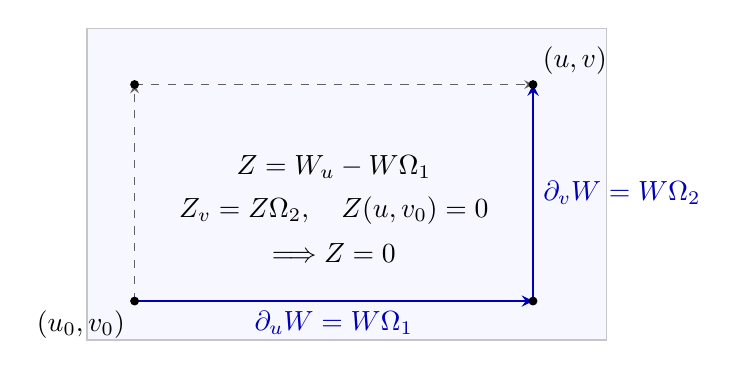
\begin{tikzpicture}[x=1.1cm,y=1.1cm,>=stealth]
	\fill[blue!3] (-0.55,-0.45) rectangle (5.45,3.15);
	\draw[gray!45] (-0.55,-0.45) rectangle (5.45,3.15);
	\draw[->,thick,blue!70!black] (0,0)--node[below] {\(\partial_uW=W\Omega_1\)} (4.6,0);
	\draw[->,thick,blue!70!black] (4.6,0)--node[right] {\(\partial_vW=W\Omega_2\)} (4.6,2.5);
	\draw[->,dashed,gray!75!black] (0,0)--(0,2.5);
	\draw[->,dashed,gray!75!black] (0,2.5)--(4.6,2.5);
	\fill (0,0) circle (1.6pt) node[below left] {\((u_0,v_0)\)};
	\fill (4.6,0) circle (1.6pt);
	\fill (0,2.5) circle (1.6pt);
	\fill (4.6,2.5) circle (1.6pt) node[above right] {\((u,v)\)};
	\node at (2.3,1.55) {\(Z=W_u-W\Omega_1\)};
	\node at (2.3,1.05) {\(Z_v=Z\Omega_2,\quad Z(u,v_0)=0\)};
	\node at (2.3,0.55) {\(\Longrightarrow Z=0\)};
\end{tikzpicture}

	\caption[矩形上的标架积分]{先沿水平线积分，再沿竖线积分。平坦性使横向误差 \(Z\) 始终为零，故交换这两个积分方向也得到同一终点标架。}
	\label{g1:fig:surface-rectangle-integration}
\end{figure}

\subsection{从标架到闭的向量值一形式}
\label{g1:subsec:0804:04}

现在假定给定数据满足 Gauss–Codazzi 条件，在任意包含基点 \(q_0=(u_0,v_0)\) 的矩形 \(V\subseteq U\) 上，用\cref{g1:lem:rectangular-matrix-system}解出初值 \(W_0\in \operatorname{SO}(3)\) 的正交标架 \(W\)，再令
\[
	\mathcal F=WP=(a_1,a_2,n).
\]
由\eqref{g1:eq:surface-orthonormal-frame-system}的定义，
\[
	\partial_i\mathcal F
	=W\Omega_iP+W\partial_iP
	=WPA_i=\mathcal F A_i.
\]
所以 \(a_1,a_2\) 已有了候选切向量应有的导数关系。还欠位置函数 \(X\)：必须证明这两个向量确实能同时写成 \(X_u,X_v\)。

\ProseParagraphBreak

把候选微分写作
\[
	\alpha=a_1\,\mathrm{d}u+a_2\,\mathrm{d}v.
\]
这是一个\term[xiangliangzhiyixingshi]{向量值一形式}[vector-valued 1-form]；这里，它将参数平面中的位移 \((\xi^1,\xi^2)\) 送到向量 \(a_1\xi^1+a_2\xi^2\)。若它的每个实分量都满足混合偏导条件，就称它为闭的；该条件写作
\[
	\mathrm{d}\alpha=(\partial_u a_2-\partial_v a_1)\,\mathrm{d}u\wedge \mathrm{d}v=0.
\]
这里 \(\mathrm{d}u\wedge \mathrm{d}v\) 只记录两个方向交换时变号；不需要预先掌握微分形式的一般理论。由 \(\partial_i\mathcal F=\mathcal F A_i\) 的前两列，
\[
	\partial_u a_2-\partial_v a_1
	=(\Gamma^1_{12}-\Gamma^1_{21})a_1
	+(\Gamma^2_{12}-\Gamma^2_{21})a_2+(h_{12}-h_{21})n=0.
\]
这一步说明了两种对称性的不同职责：Gauss–Codazzi 条件先使标架能够积分，而 \(\Gamma^k_{12}=\Gamma^k_{21}\)、\(h_{12}=h_{21}\) 再使位置的候选微分闭合。两步缺一不可。

\subsection{浸入的构造和秩检验}
\label{g1:subsec:0804:05}

在矩形上，把闭的向量值一形式积分成位置无需调用另一个一般存在定理。指定 \(x_0\in\mathbb R^3\)，直接沿刚才的折线定义
\begin{equation}
	\label{g1:eq:surface-position-rectangle-integral}
	X(u,v)=x_0+\int_{u_0}^u a_1(s,v_0)\,\mathrm{d}s+\int_{v_0}^v a_2(u,t)\,\mathrm{d}t.
\end{equation}
对 \(v\) 求导得到 \(X_v=a_2\)。对 \(u\) 求导，并用 \(\partial_u a_2=\partial_v a_1\)，得到
\[
	X_u=a_1(u,v_0)+\int_{v_0}^v\partial_u a_2(u,t)\,\mathrm{d}t
	=a_1(u,v_0)+a_1(u,v)-a_1(u,v_0)=a_1(u,v).
\]
于是 \(\mathrm{d}X=\alpha\)，且 \(X(q_0)=x_0\)。积分中各函数光滑，故 \(X\) 光滑。

\ProseParagraphBreak

有了位置函数还不能直接宣布它是正则曲面，必须检查两个切向量处处独立。由 \(W^{\mathsf T}W=I\) 及 \(P^{\mathsf T}P=\mathcal G\)，对任意 \(\xi=(\xi^1,\xi^2)\in\mathbb R^2\)，
\[
	\|\mathrm{d}X(\xi)\|^2
	=\|a_1\xi^1+a_2\xi^2\|^2
	=g_{ij}\xi^i\xi^j.
\]
当 \(\xi\ne0\) 时，正定性使右端严格为正，因此 \(\mathrm{d}X\) 的核为零、秩为 \(2\)。这正是最初坚持 \(g\) 正定的原因；若它退化，即使所有偏导相容，也不能保证得到浸入。

\subsection{两基本形式的恢复}
\label{g1:subsec:0804:06}

构造出了浸入，还须核对它实现的是原先的数据。第一基本形式由 \(\mathcal F^{\mathsf T}\mathcal F=\mathcal G\) 立即得到：
\[
	\langle X_i,X_j\rangle=\langle a_i,a_j\rangle=g_{ij}.
\]
从\eqref{g1:eq:surface-metric-factor}的列向量关系得到
\[
	X_u\times X_v=a_1\times a_2=\sqrt D\,n,
\]
故标架第三列确实等于按参数顺序选择的单位法向 \((X_u\times X_v)/\|X_u\times X_v\|\)。取 \(\partial_i\mathcal F=\mathcal F A_i\) 的第 \(j\) 列，
\[
	X_{ij}=\Gamma^1_{ij}X_u+\Gamma^2_{ij}X_v+h_{ij}n.
\]
与 \(n\) 作内积即得 \(\langle X_{ij},n\rangle=h_{ij}\)，所以第二基本形式也恢复了。特别地，第二基本形式的符号并非由事后任取法向决定；构造中的 \(P\) 和 \(W\in \operatorname{SO}(3)\) 已使它与给定参数方向一致。

\begin{example}[平直度量配上非零弯曲]
	\label{g1:exm:fundamental-cylinder-data}
	取 \(g=\mathrm{d}u^2+\mathrm{d}v^2\)、\(h=\lambda\,\mathrm{d}u^2\)，其中 \(\lambda\ne0\) 为常数。此时 \(\Gamma=0\)、\(K_g=0\)、\(\det h=0\)，Codazzi 条件也因系数常数而成立。取 \(P=I\)、\(W(0,0)=I\)，系统成为
	\[
		A_1=\begin{pmatrix}0&0&-\lambda\\0&0&0\\\lambda&0&0\end{pmatrix},
		\qquad A_2=0.
	\]
	于是
	\[
		a_1=(\cos\lambda u,0,\sin\lambda u),\quad
		a_2=(0,1,0),\quad n=(-\sin\lambda u,0,\cos\lambda u).
	\]
	以 \(X(0,0)=0\) 积分，得到
	\[
		X(u,v)=\left(\frac{\sin\lambda u}{\lambda},\,v,\,
		\frac{1-\cos\lambda u}{\lambda}\right).
	\]
	这是半径 \(1/|\lambda|\) 的圆柱面参数化。平直的长度数据允许一个切向方向发生弯曲；Gauss 方程只要求两个主曲率的乘积为零，并不要求每个主曲率都为零。
\end{example}

\subsection{局部唯一性与整体单值}
\label{g1:subsec:0804:07}

现在把构造和唯一性合并成完整结论。初始标架所规定的是两个切向量按顺序正交归一化后的方向，而不是任意指定 \(X_u,X_v\) 的长度；后者已由 \(g\) 给定。

\begin{theorem}[曲面基本定理]
	\label{g1:thm:surface-fundamental}
	设 \(U\subseteq\mathbb R^2\) 为开集，\(g=(g_{ij})\) 为光滑正定对称矩阵，\(h=(h_{ij})\) 为光滑对称矩阵，各矩阵均为 \(2\times2\)。令 \((g^{ij})=g^{-1}\)，\(\Gamma\) 为 \(g\) 的 Christoffel 系数，\(\nabla_i\partial_j=\Gamma^k_{ij}\partial_k\)，\(R\) 为该联络的曲率，约定 \(R(V,W)Z=\nabla_V\nabla_WZ-\nabla_W\nabla_VZ-\nabla_{[V,W]}Z\)。以 \(R(\partial_1,\partial_2)\partial_j=R^k{}_{j12}\partial_k\) 定义分量，令 \(h_i{}^k=g^{k\ell}h_{i\ell}\)、\(\nabla_i h_{jk}=\partial_i h_{jk}-\Gamma^\ell_{ij}h_{\ell k}-\Gamma^\ell_{ik}h_{j\ell}\)，要求 \(R^k{}_{j12}=h_1{}^kh_{2j}-h_2{}^kh_{1j}\) 及 \(\nabla_1h_{2j}=\nabla_2h_{1j}\) 对 \(j,k=1,2\) 成立，即\eqref{g1:eq:surface-data-gauss}、\eqref{g1:eq:surface-data-codazzi}。令 \(E=g_{11}\)、\(F=g_{12}\)、\(D=\det g\)，并令 \(P=\begin{psmallmatrix}\sqrt E&F/\sqrt E&0\\0&\sqrt D/\sqrt E&0\\0&0&1\end{psmallmatrix}\)。给定 \(q_0=(u_0,v_0)\in U\)、\(x_0\in\mathbb R^3\) 及右手正交标架矩阵 \(W_0\in\operatorname{SO}(3)\)，则在每个含 \(q_0\) 的开矩形 \(V\subseteq U\) 上，存在唯一的光滑浸入 \(X\colon V\rightarrow\mathbb R^3\)，其第一、第二基本形式分别为 \(g,h\)，且
	\[
		X(q_0)=x_0,\qquad
		(X_u,X_v,n)(q_0)=W_0P(q_0),\qquad
		n=\frac{X_u\times X_v}{\|X_u\times X_v\|}.
	\]
	这里 \(P\) 由\eqref{g1:eq:surface-metric-factor}确定。若不指定这些初值，同一矩形上的任意两个这样的浸入满足
	\[
		\widetilde X=QX+b,\qquad Q\in \operatorname{SO}(3),\quad b\in\mathbb R^3.
	\]
	这一结论称为\term[qumianjibendingli]{曲面基本定理}[fundamental theorem of surface theory]。
\end{theorem}

\begin{proof}
	由\cref{g1:prop:surface-data-flatness}及\eqref{g1:eq:surface-flatness-change-frame}，\(\Omega_1,\Omega_2\) 满足平坦性；它们的斜对称性已由\eqref{g1:eq:surface-matrix-metric-compatibility}证明。\cref{g1:lem:rectangular-matrix-system}给出初值为 \(W_0\) 的 \(\operatorname{SO}(3)\) 值解。于是前面三小节的构造依次给出闭的候选微分、\eqref{g1:eq:surface-position-rectangle-integral}中的光滑浸入，以及其基本形式和法向的逐项核验，这证明存在性。

	对于任意另一个具有相同数据的浸入 \(\widetilde X\)，\cref{g1:prop:gauss-weingarten}使其坐标标架 \(\widetilde{\mathcal F}=(\widetilde X_u,\widetilde X_v,\widetilde n)\) 满足相同的 \(\partial_i\widetilde{\mathcal F}=\widetilde{\mathcal F}A_i\)。因 \(g\) 相同，\(\widetilde W=\widetilde{\mathcal F}P^{-1}\) 满足同一正交标架系统。若初值也相同，矩形积分引理的唯一性给出 \(\widetilde W=W\)，从而 \(\mathrm{d}\widetilde X=\mathrm{d}X\)。两者之差的两个偏导都为零，沿水平、竖直线段积分可知其在矩形上为常数；基点位置相同便使这个常数为零。

	若不指定初值，令 \(Q=\widetilde W(q_0)W(q_0)^{\mathsf T}\in \operatorname{SO}(3)\)。矩阵 \(QW\) 满足与 \(\widetilde W\) 相同的系统和初值，因此 \(\widetilde W=QW\)。于是 \(\mathrm{d}\widetilde X=Q\,\mathrm{d}X\)，积分得到 \(\widetilde X=QX+b\)，其中 \(b=\widetilde X(q_0)-QX(q_0)\)。
\end{proof}

这里的“唯一”保留了参数点之间的对应；若允许重新参数化，就必须同时按该坐标变换拉回 \(g,h\)。此外，保向刚性变换的限定与法向约定有关：若用一个行列式为 \(-1\) 的正交矩阵反射曲面，按参数叉积重新选择的法向会多出一个负号，第二基本形式随之变号。

\ProseParagraphBreak

对一般开集，定理保证每点附近的局部实现。若沿一条道路继续这些局部解，相交处可用同一位置和标架初值保证它们一致；每一段有限道路只需有限多个小矩形。但绕环路回来时，标架可能已经转动，或者标架虽回到原值，位置却发生平移。这与\cref{g1:prop:periodic-curve-closure}中“标架回到初值”和“位移积分为零”两个条件的区别相同。以下两个例子直接显示这两种障碍，而不把局部存在性误当成任意区域上的单值存在性。

\begin{example}[转动障碍与位移障碍]
	\label{g1:exm:surface-monodromy-obstructions}
	在环带 \(A=\{(x,y):1<\sqrt{x^2+y^2}<2\}\) 上，写 \(r=\sqrt{x^2+y^2}\)。角度 \(\theta\) 不是整个环带上的单值实函数，但
	\[
		\mathrm{d}r=\frac{x\,\mathrm{d}x+y\,\mathrm{d}y}{r},\qquad
		\mathrm{d}\theta=\frac{-y\,\mathrm{d}x+x\,\mathrm{d}y}{r^2}
	\]
	都是单值的一形式；局部选定角度后，它们就是通常的坐标微分。

	先取 \(g=\mathrm{d}r^2+c^2r^2\mathrm{d}\theta^2\)、\(h=0\)，其中 \(c>0\)。在展开角度的矩形 \((1,2)\times\mathbb R\) 上，
	\[
		\widetilde X(r,\theta)=(r\cos c\theta,r\sin c\theta,0)
	\]
	实现这两组数据，因而各局部坐标中的 Gauss–Codazzi 条件都成立。它的单位径向、角向标架绕一周后旋转 \(2\pi c\)。若 \(c\notin\mathbb Z\)，这个标架不能在 \(\theta\) 与 \(\theta+2\pi\) 处匹配。假如环带上有实现数据的单值浸入，把它写到展开角度的矩形上，再用曲面基本定理的唯一性，它必与 \(\widetilde X\) 相差固定保向刚性变换；但固定刚性变换不能消除标架的不匹配，故这样的浸入不存在。

	再取 \(g=\mathrm{d}r^2+\mathrm{d}\theta^2\)、\(h=0\)。在展开角度的矩形上，\(\widetilde X(r,\theta)=(r,\theta,0)\) 实现数据，沿径向、角向的标架都是常向量，已经没有转动障碍。然而候选位置微分为 \(\alpha=(\mathrm{d}r,\mathrm{d}\theta,0)\)，沿任一正向圆周积分得到
	\[
		\oint\alpha=(0,2\pi,0)\ne0.
	\]
	一个单值位置函数的微分沿环路积分必须等于终点减起点，即零；这里却存在非零位移。也可直接由 \(\widetilde X(r,\theta+2\pi)-\widetilde X(r,\theta)=(0,2\pi,0)\) 和同样的唯一性论证排除整体浸入。
\end{example}

这两个例子中的数据处处光滑并且满足相容方程，障碍只在绕环带一周后出现。因而 Gauss–Codazzi 方程精确回答了局部能否实现的问题；在带孔区域上还要另查标架运输和环路位移，不能仅检查点上的曲率等式。
